\documentclass{if-beamer}

% --------------------------------------------------- %
%                  Presentation info	              %
% --------------------------------------------------- %
\title[Projeto -- Etapa 1]{Arquitetura HIL para teste de sistemas embarcados como \textit{vehicle interfaces} de veículos autônomos baseados no Autoware}
\subtitle{Projeto -- Etapa 1}

\author[Gabriel Toffanetto]{Gabriel Toffanetto França da Rocha 
	\\ \vspace{1mm} 
	\small{\href{mailto:g289320@dac.unicamp.br}{g289320@dac.unicamp.br}}
}

\institute[LMA/FEM/Unicamp]{\small{Professor Dr. Rodrigo Moreira Bacurau
  \\ \vspace{2mm}
  IM420X -- Projeto de Sistemas Embarcados de Tempo Real
  \\ \vspace{4mm}
  Faculdade de Engenharia Mecânica
  \\ \vspace{1mm}
  Universidade Estadual de Campinas}
}

\date{8 de outubro de 2024}

\logo{
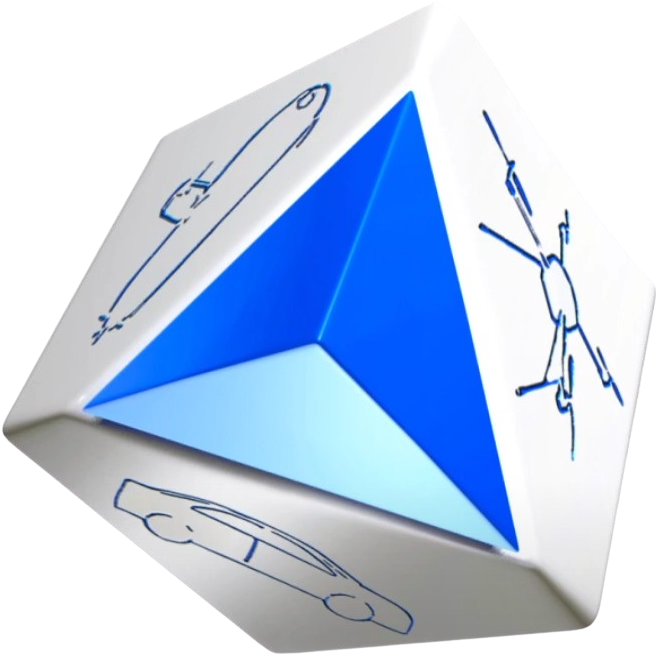
\includegraphics[width=1.2cm]{img/core/Logo_LMA_icon.png}
}


\subject{IM420X - Projeto final etapa 1} % metadata

\graphicspath{{img/}}

\setbeamertemplate{caption}[numbered]

\newcolumntype{b}{>{\columncolor{white}}c}


% --------------------------------------------------- %
%                    Title + Schedule                 %
% --------------------------------------------------- %

\begin{document}

\begin{frame}
  \titlepage
\end{frame}

\begin{frame}{Schedule}
  \tableofcontents
\end{frame}

% --------------------------------------------------- %
%                      Presentation                   %
% --------------------------------------------------- %

\section{Introdução}

\begin{frame}{Contextualização}
	
	\begin{columns}
		
		\begin{column}{0.4\textwidth}
			
		
			\begin{figure}[H]
				\centering
				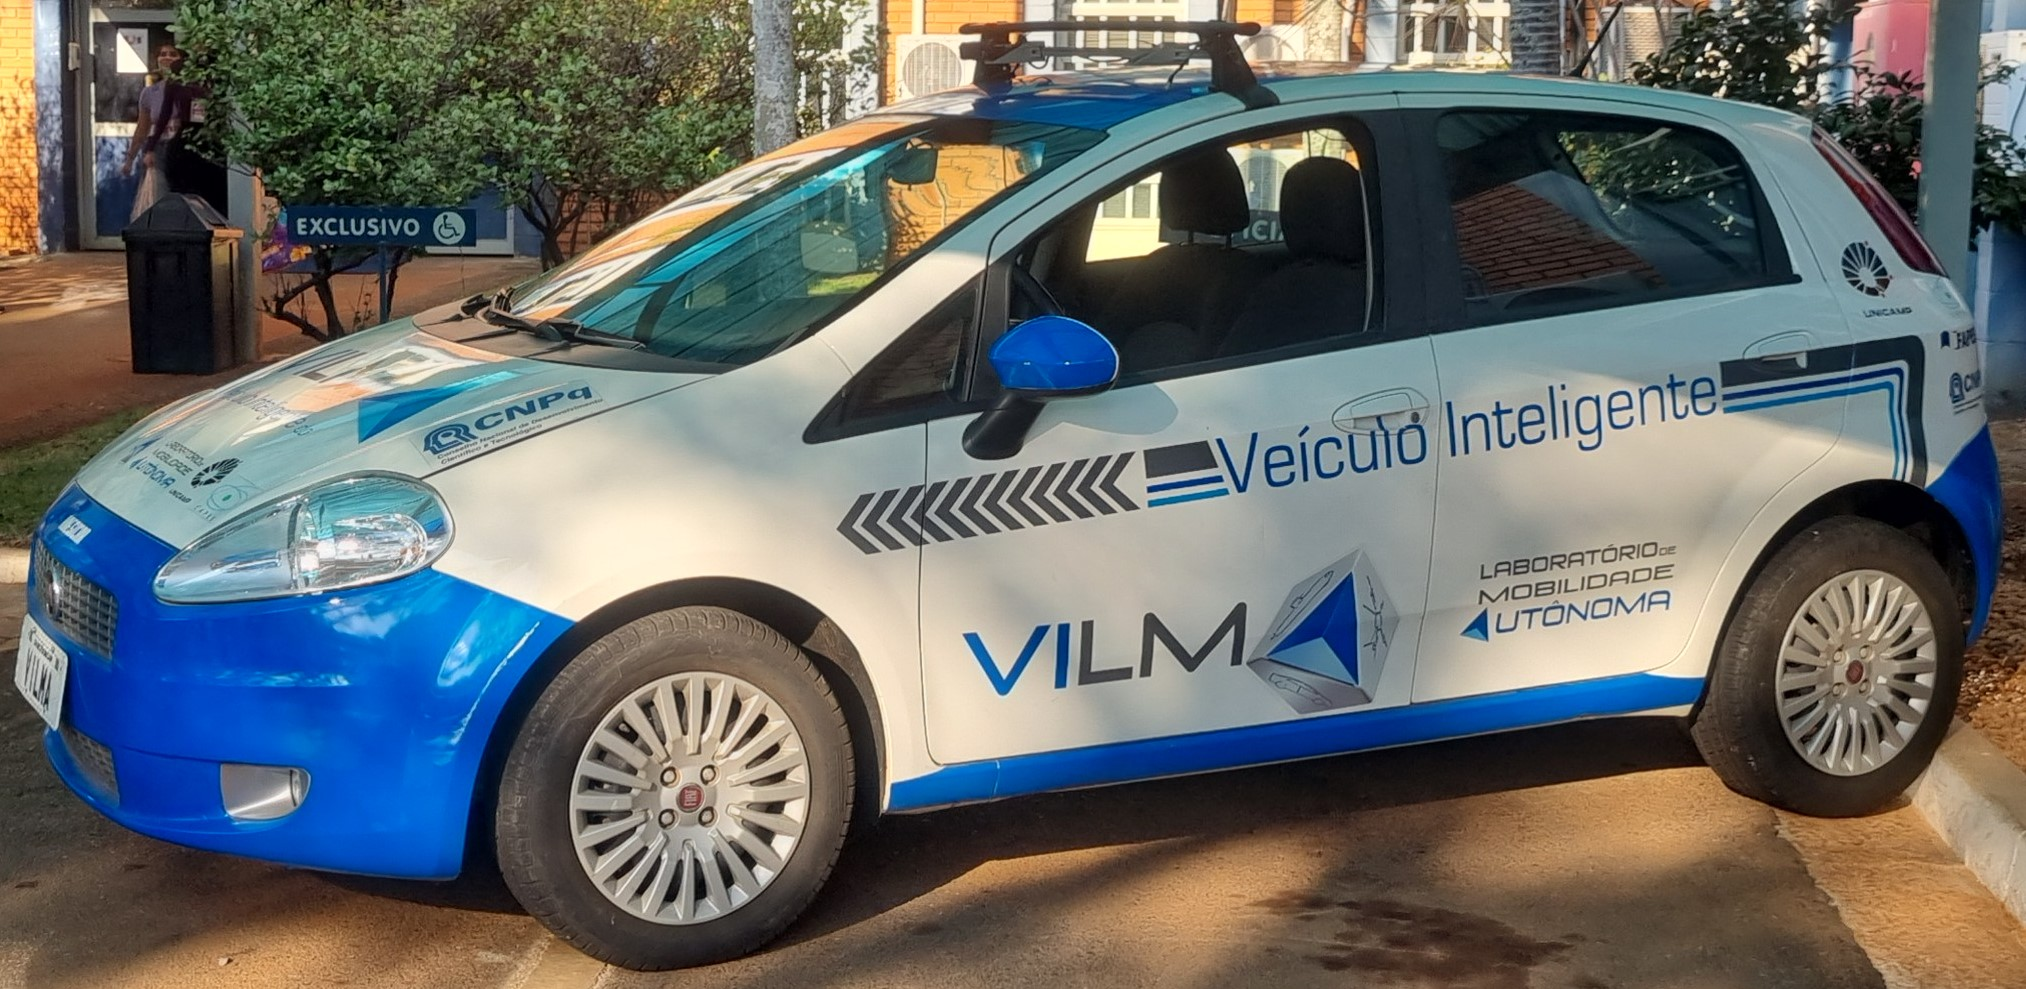
\includegraphics[width=\linewidth]{img/vilma}
				\caption{Veículo Autônomo do LMA.}
				\label{fig:vilma}
			\end{figure}
		\end{column}
	
		\begin{column}{0.6\textwidth}
		
		\begin{figure}[H]
			\centering
			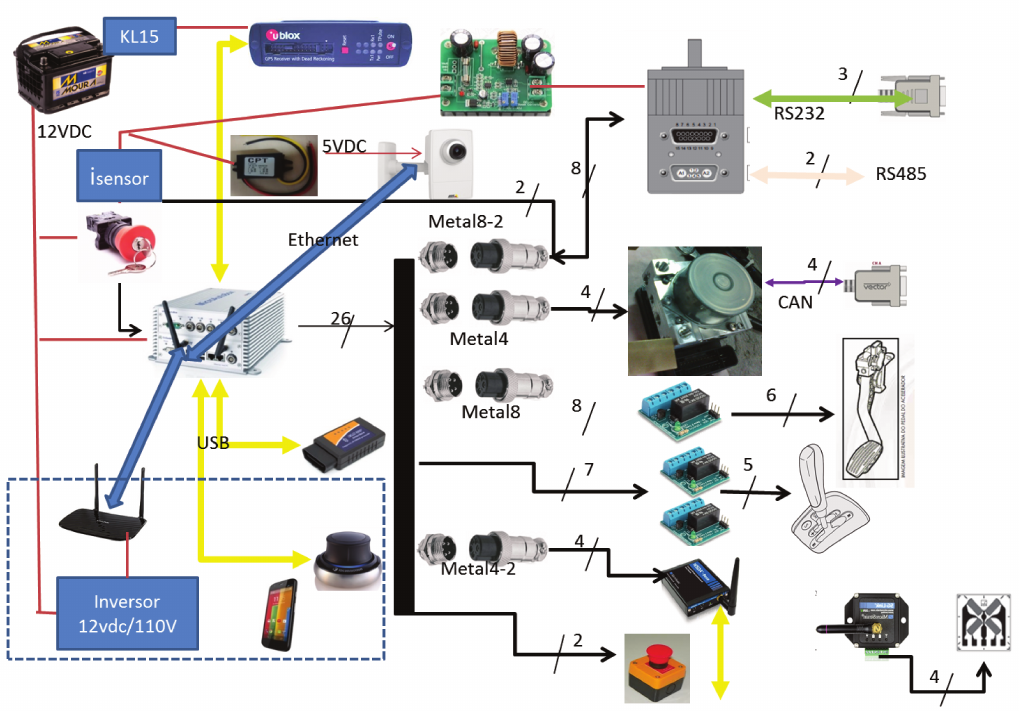
\includegraphics[width=1\linewidth]{img/diagrama_vilma}
			\caption{Diagrama de \textit{hardware} do VILMA01 \cite{bedoya_alise_2016}.}
			\label{fig:diagrama_vilma}
		\end{figure}
		
		\end{column}
		
	\end{columns}
	
	
	
\end{frame}

\subsection*{Autoware}

\begin{frame}{Autoware}
	
	\begin{block}{O que é?}
		\begin{itemize}
			\item Projeto de \textit{software open-source} que consiste em todas as funcionalidades requeridas para condução autônoma, em uma arquitetura modular com interfaces e APIs bem definidas;
			\item Primeiro "\textit{all-in-one}" \textit{open-source software} para veículos autônomos.
		\end{itemize}
	\end{block}
	
	\begin{block}{Princípios}
		\begin{itemize}
			\item Projetado para suprir as necessidades de diferentes aplicações autônomas;
			\item Desenvolvido com as melhores práticas e padrões para alcançar alta qualidade e segurança em produtos para o mundo real.
		\end{itemize}
	\end{block}
	
	\boxblue[0.6]{
		\centering
		\textbf{"Autoware continuously evolves to offer more capability towards curb-to-curb Level 4 autonomous driving."}
	}
	
\end{frame}

\begin{frame}{Arquitetura}
	
	% TODO: \usepackage{graphicx} required
	\begin{figure}
		\centering
		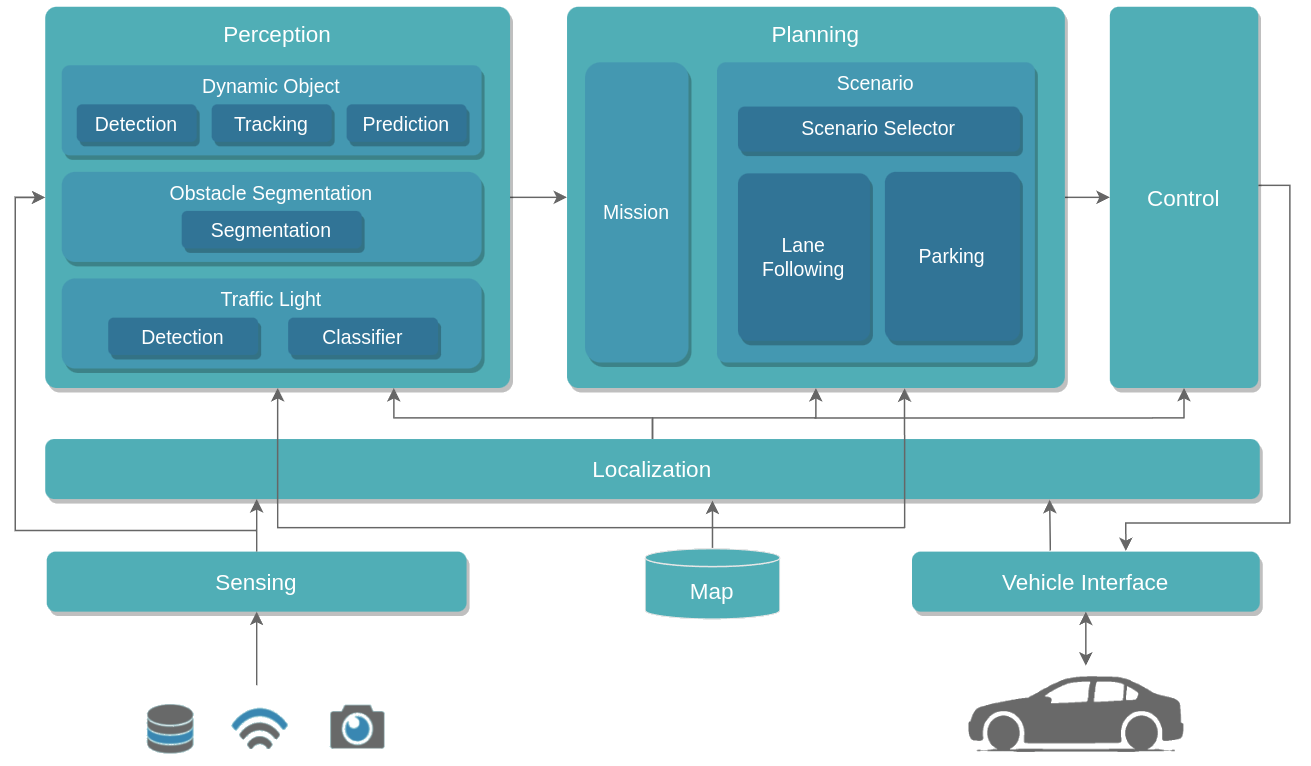
\includegraphics[width=1\linewidth]{img/HL_architecture}
		\caption{Arquitetura de alto nível \cite{autowareArchitecture}.}
		\label{fig:hlarchitecture}
	\end{figure}
	
\end{frame}

\subsection*{ROS}

\begin{frame}{ROS -- \textit{Robot Operation System}}
	
	\begin{block}{O que é?}
		\begin{itemize}
			\item \textit{Framework} para robótica que contempla toda estrutura que um robô precisa;
			\begin{itemize}
				\item Ferramentas e bibliotecas;
				\item Protocolos de comunicação;
				\item Interfaceamento.
				
			\end{itemize}
			\item Arquitetura baseada em sistema distribuído (ROS 2);
			\item Alta modularização com reaproveitamento de código próprio ou da comunidade;
			\item Portabilidade simulação/\textit{hardware}.
		\end{itemize}
	\end{block}
	
	
% TODO: \usepackage{graphicx} required
\begin{figure}
	\centering
	
\includegraphics[width=1\linewidth]{img/ros-equation.png}
	\caption{Ecossitema ROS \cite{ecoros}.}
	\label{fig:ros-equation}
\end{figure}
	
\end{frame}


\subsection*{micro-ROS}

\begin{frame}{micro-ROS}
	
	\begin{block}{O que é?}
		\begin{itemize}
			\item \textit{Framework} que leva o ROS 2 à microcontroladores.
		\end{itemize}
	\end{block}
	
	% TODO: \usepackage{graphicx} required
	\begin{figure}
		\centering
		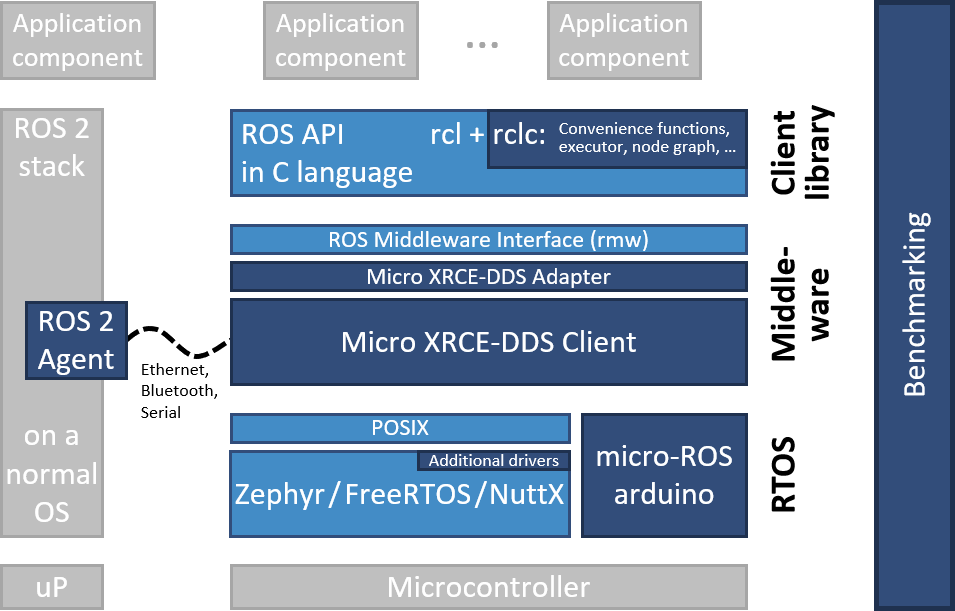
\includegraphics[width=0.7\linewidth]{img/micro-ROS_architecture}
		\caption{Arquitetura micro-ROS \cite{microros}.}
		\label{fig:micro-rosarchitecture}
	\end{figure}
	
	
	
\end{frame}

\section{Proposta}

\begin{frame}{Proposta}
	
\Wider{
	
	\begin{columns}
		
		\begin{column}{0.55\textwidth}
			
				\begin{figure}[H]
				\centering
				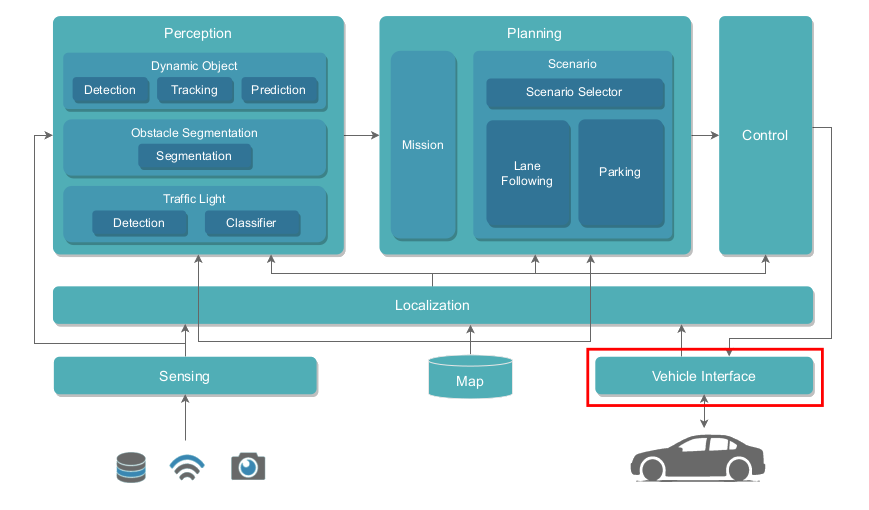
\includegraphics[width=\linewidth]{img/architecture.png}
				\caption{Escopo do projeto na arquitetura Autoware.}
				\label{fig:architecture}
			\end{figure}
			
		\end{column}
		
		\begin{column}{0.45\textwidth}
			
				\begin{figure}[H]
				\centering
				\includegraphics[width=\linewidth]{img/architecture_HIL}
				\caption{Arquitetura de teste do \textit{hardware}.}
				\label{fig:architecture_HIL}
			\end{figure}
			
		\end{column}
		
	\end{columns}
	
}
	
\end{frame}

\begin{frame}{Proposta}
	
	\begin{block}{Objetivos}
		
		\begin{itemize}
			\item Desenvolvimento de um sistema embarcado capaz de agir como \textit{vehicle interface} para um veículo autônomo compatível com o Autoware utilizando o micro-ROS;
			\item Teste do sistema embarcado por meio de \textit{Hardware-In-the-Loop} com o simulador CARLA ou AWSIM.
			
		\end{itemize}
		
	\end{block}
	
	\begin{block}{Justificativa}
	
	\begin{itemize}
		\item O Autoware é um sistema para carros autônomos em ascensão, sendo importante que sistemas embarcados presentes nesses veículos sejam capazes de se integrar com ele. Dessa forma, a proposta da implementação de um sistema embarcado como \textit{vehicle interface} garante a interligação entre microcontroladores STM32 ao \textit{framework}. A validação por meio de HIL se faz interessante por substituir a necessidade de um protótipo real para testes, garantindo mais segurança, praticidade e redução de custos no desenvolvimento do projeto.
		
	\end{itemize}
	
	\end{block}
	
\end{frame}

\begin{frame}{Requisitos}
	
	\begin{columns}
		
		\begin{column}{0.5\textwidth}
			
			\begin{block}{Requisitos funcionais}
				
				\begin{itemize}
					\item Comunicação com o Autoware;
					\item Controle da aceleração, frenagem e direção do veículo;
					\item Controle dos faróis e luzes de sinalização (seta) do veículo;
					\item Teleoperação do veículo por um \textit{joystick} em  \textit{hardware}.
					
				\end{itemize}
				
			\end{block}
			
		\end{column}
		
		\begin{column}{0.5\textwidth}
			
			\begin{block}{Requisitos não-funcionais}
				
				\begin{itemize}
					\item A \textit{vehicle interface} deve ser construída na forma de um pacote portável para outros microcontroladores STM32;
					\item O interfaceamento com o veículo deve ser intercambiável com diferentes configurações;
					\item Deve-se garantir sincronização de \textit{timestamp} entre o Autoware e o microcontrolador;
					\item O sistema embarcado deve abstraír o veículo como um sistema \textit{Drive-By-Wire} (DBW) para o Autoware.
				\end{itemize}
				
			\end{block}
			
		\end{column}
		
	\end{columns}
	
	
\end{frame}


\begin{frame}{Componentes}
	
		\begin{columns}
		
		\begin{column}{0.6\textwidth}
			
	\begin{block}{Placa de desenvolvimento NUCLEO-H753ZI}
	
	\begin{itemize}
		\item Microcontrolador STM32H753ZI;
		\item ARM Cortex-M7;
		\item 1 MB RAM;
		\item 2 MB Flash;
		\item 480 MHz (max) CPU;
		\item DMA;
		\item Comunicação:
		\begin{itemize}
			\item UART/USART;
			\item Ethernet;
			\item USB.
		\end{itemize}
		\item Custo: US\$ 27,00.
	\end{itemize}
	
\end{block}
			
		\end{column}
		
		\begin{column}{0.4\textwidth}
			
			\begin{figure}[H]
				\centering
				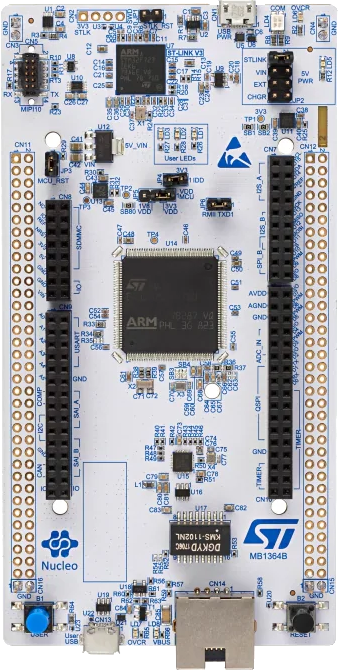
\includegraphics[width=0.7\linewidth]{img/nucleo}
				\caption{NUCLEO-753ZI.}
				\label{fig:nucleo}
			\end{figure}
			
		\end{column}
		
	\end{columns}
	

\end{frame}


\begin{frame}{Componentes}
	
	\begin{columns}
		
		\begin{column}{0.6\textwidth}
			
			\begin{block}{Joystick}
				
				\begin{itemize}
					\item Tensão de operação: 3V3 -- 5V;
					\item Saída analógica referente ao eixo $x$;
					\item Saída analógica referente ao eixo $y$;
					\item Saída digital referente ao eixo $z$;
					\item Custo: R\$ 10,00.
				\end{itemize}
				
			\end{block}
			
		\end{column}
		
		\begin{column}{0.4\textwidth}
			
			\begin{figure}[H]
				\centering
				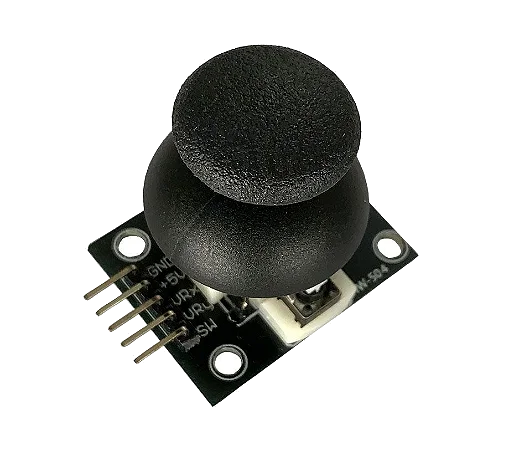
\includegraphics[width=0.9\linewidth]{img/joystick}
				\caption{Joystick 2 eixos.}
				\label{fig:joystick}
			\end{figure}
			
		\end{column}
		
	\end{columns}
	
	
\end{frame}


\section{Arquitetura}

\begin{frame}{Diagrama de blocos}


	\begin{figure}
		\centering
		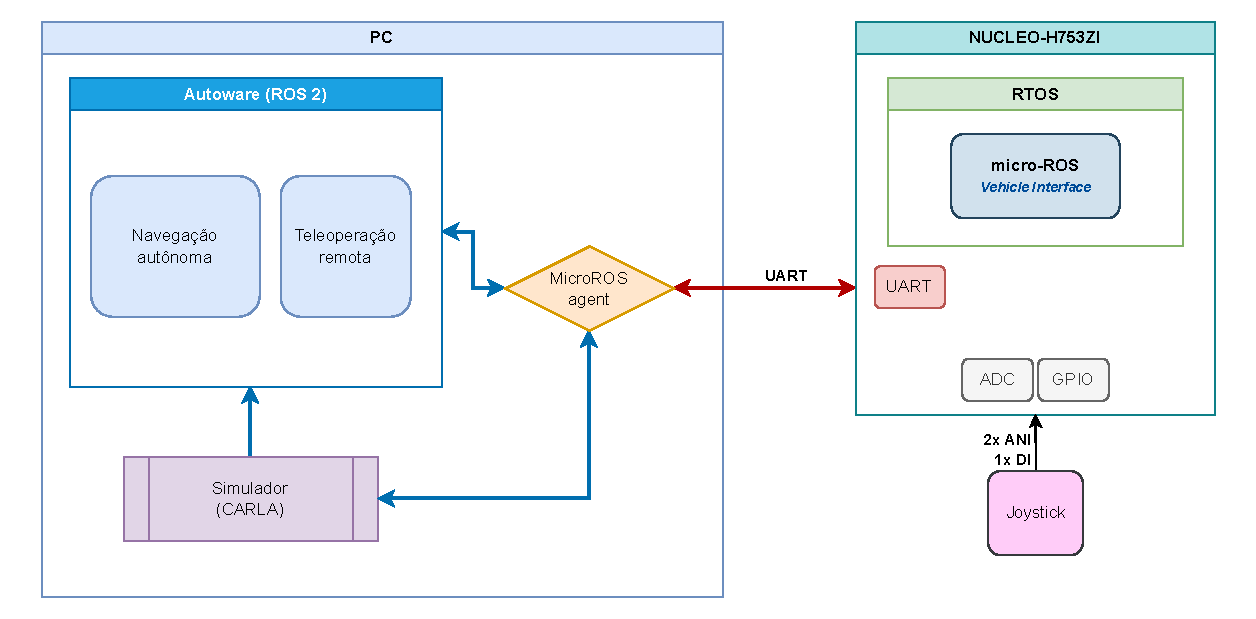
\includegraphics[width=\linewidth]{img/block_diagram.pdf}
		\caption{Diagrama de blocos da arquitetura HIL.}
		\label{fig:blockdiagram}
	\end{figure}
	

\end{frame}


\begin{frame}{Esquemático}
	
		
	\begin{figure}
		\centering
		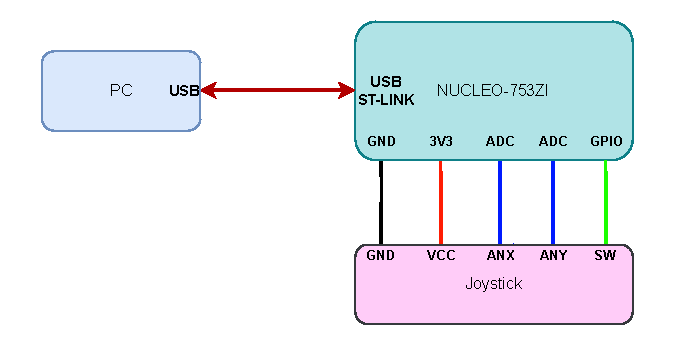
\includegraphics[width=\linewidth]{img/esquematico.pdf}
		\caption{Esquemático de ligações elétricas.}
		\label{fig:esquematico}
	\end{figure}
	
\end{frame}



\section{Cronograma}

\begin{frame}{Modelo de desenvolvimento}
	
	
	\begin{block}{Modelo V}
		
		\begin{itemize}
			\item Realização e validação de cada etapa do projeto em paralelo.
			
		\end{itemize}
		
	\end{block}
	
	
	% TODO: \usepackage{graphicx} required
	\begin{figure}
		\centering
		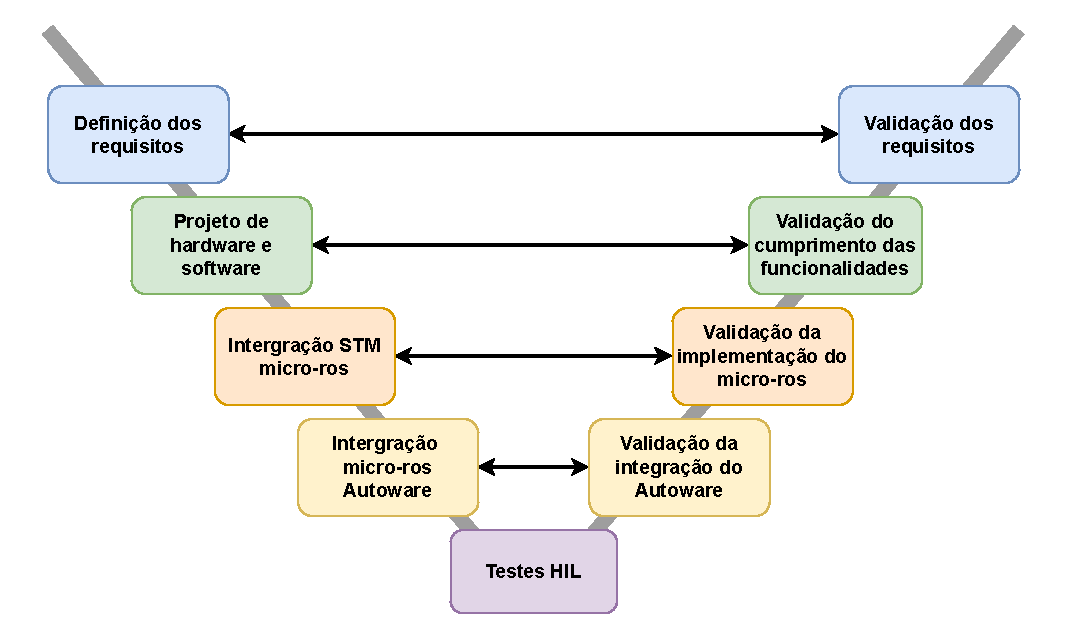
\includegraphics[width=0.8\linewidth]{img/modelo-v}
		\caption{Modelo de execução das atividades do projeto.}
		\label{fig:modelo-v}
	\end{figure}

	
\end{frame}

\begin{frame}{Cronograma}
	
\Wider{
	
	
\begin{table}
	\centering
	\small{
		\begin{tabular}{|b|b|b|b|b|b|b|b|b|b|}
			\hline
			\textbf{Atividade/Semana} & 1 & \textbf{2} & 3 & \textbf{4} & 5 & 6 & \textbf{7} & 8 & \textbf{9} \\
			\hline
			Proposta do projeto  & \cellcolor{unifeiblue} &  &  &  &  &  &  &  &  \\
			\hline
			Projeto de \textit{hardware} e \textit{software}  &  & \cellcolor{unifeiblue} & \cellcolor{unifeiblue} &  &  &  &  &  &  \\
			\hline
			Integração do STM com o micro-ROS  &  & \cellcolor{unifeiblue} &  &  &  &  &  &  &  \\
			\hline
			Integração do micro-ROS com o Autoware  &  &  & \cellcolor{unifeiblue} & \cellcolor{unifeiblue} &  &  &  &  &  \\
			\hline
			Implementação das tarefas do sistema embarcado  &  &  &  & \cellcolor{unifeiblue} & \cellcolor{unifeiblue} & \cellcolor{unifeiblue} & \cellcolor{unifeiblue} &  &  \\
			\hline
			Construção do ambiente de testes  &  &  &  &  & \cellcolor{unifeiblue} & \cellcolor{unifeiblue} & \cellcolor{unifeiblue} &  &  \\
			\hline
			Realização dos testes  &  &  &  &  &  &  & \cellcolor{unifeiblue} & \cellcolor{unifeiblue} & \cellcolor{unifeiblue} \\
			\hline
			Escrita do relatório  &   & \cellcolor{unifeiblue} & \cellcolor{unifeiblue} & \cellcolor{unifeiblue} & \cellcolor{unifeiblue} & \cellcolor{unifeiblue} & \cellcolor{unifeiblue} & \cellcolor{unifeiblue} & \cellcolor{unifeiblue} \\
			\hline
		\end{tabular}
	}
	\caption{Cronograma de atividades.}
	\label{tab:crono}
\end{table}

}
	
	\begin{itemize}
		\small
		\item \textbf{Semana 2:} Apresentação Etapa 1
		\item \textbf{Semana 4:} Apresentação Etapa 2
		\item \textbf{Semana 7:} Apresentação Etapa 3
		\item \textbf{Semana 9:} Apresentação Final
	\end{itemize}
	
\end{frame}


% -------------------------------------------------
%               Bibliografia.
%--------------------------------------------------
\section{Referências bibliográficas}
\begin{frame}{Referências bibliográficas}
   %\bibliographystyle{acm}
   \bibliography{bibliografia.bib}
\end{frame}

\end{document}
